\newpage
\criteria{Teaching and Learning Approach}

\subcriteria{The educational philosophy is shown to be articulated and communicated to all stakeholders. It is also shown to be reflected in the teaching and learning activities.}

ปรัชญาการศึกษาของมหาวิทยาลัย \textbf{นวัตกรรมสร้างชาติ ราชมงคลธัญบุรีสร้างนวัตกรรม}

คณะฯ มีการชี้แจงนโยบายการจัดการเรียนการสอนโดยนำปรัชญาการศึกษามาเป็นแนวทางการจัดการเรียนการสอนผ่านการประชุมคณะกรรมการบริหารคณะ/การประชุมคณาจารย์ภายในคณะ จากนั้นหลักสูตรได้สื่อสารปรัชญาการศึกษากับอาจารย์ผู้สอนให้รับทราบแนวทางการจัดการเรียนการสอนที่มุ่งเน้นการพัฒนาบัณฑิตสู่การเป็นนวัตกร ผ่านการประชุมอาจารย์ผู้รับผิดชอบหลักสูตร และอาจารย์ผู้สอน 

หลักสูตรได้กำหนดให้อาจารย์ผู้รับผิดชอบรายวิชาและอาจารย์ผู้สอนนำปรัชญาการศึกษาของมหาวิทยาลัยมาใช้ในการจัดการเรียนการสอนเพื่อพัฒนาบัณฑิตสู่การเป็นนวัตกร โดยมุ่งเน้นให้ผู้เรียนได้ปฏิบัติจริงและพัฒนาทักษะกระบวนการคิด ในรูปแบบของ active learning  ที่หลากหลายในทุกรายวิชาชีพที่เปิดสอนให้กับนักศึกษาในหลักสูตร ทั้งนี้ ขึ้นอยู่กับความเหมาะสมของรายวิชา เช่น Problem-based Learning, Project-based Learning, Activity-based Learning และ Case-based Learning  พร้อมทั้งมีการใช้เทคนิคการสอนสมัยใหม่ เช่น CDIO STEM, FINLAND Model, Problem Based หรืออื่นๆ ในการจัดการเรียนการสอน รวมถึงมีการฝึกสหกิจศึกษา/ฝึกงาน ในสถานประกอบการ 

หลักสูตรมีการสื่อสารปรัชญาการศึกษากับนักศึกษาผ่านอาจารย์ที่ปรึกษาในกิจกรรม Home room/การจัดการเรียการสอนในแต่ละรายวิชา นอกจากนั้นหลักสูตรยังมีการสื่อสารปรัชญาการศึกษากับนักเรียน/นักศึกษาที่จะมาเรียนในหลักสูตรในอนาคตผ่านการประชาสัมพันธ์หลักสูตร เช่น เว็บไซต์คณะ เว็บไซต์สาขาวิชา แผ่นพับ เป็นต้น

%\newpage
\begin{doclist}
	\docitem{รายงานการประชุมอาจารย์ผู้รับผิดชอบหลักสูตรและอาจารย์ผู้สอน
	เพื่อสื่อสารปรัชญาการศึกษา และนำปรัชญาการศึกษามาใช้ในการจัดการเรียนการสอน}
	%\docitem{การสื่อสารปรัชญาการศึกษากับนักศึกษา}
	%\docitem{ช่องทางการสื่อสารกับผู้มีส่วนได้ส่วนเสีย}
\end{doclist}

\subcriteria{The teaching and learning activities are shown to allow students to participate responsibly in the learning process.}
หลักสูตรมีการจัดการเรียนการสอนเพื่อให้ผู้เรียนมีส่วนร่วมในกระบวนการจัดการเรียนรู้ โดยให้นักศึกษามีส่วนร่วมแบบรับผิดชอบในกระบวนการการเรียนการสอนร่วมกับอาจารย์  ประเมินเพื่อนร่วมกับอาจารย์ในการนำเสนอ การสร้างชิ้นงาน กำหนดรูปแบบการเรียนการสอน การวางแผนการเรียนร่วมกัน เช่น รายวิชาทฤษฎีจำนวนและการประยุกต์
วันแรกของการเปิดภาคการศึกษา อาจารย์ได้ชี้แจงประมวลรายวิชา พูดถึงภาพรวมของรายวิชา คำอธิบายรายวิชา เกณฑ์การวัดและประเมินผล แผนการสอนในแต่ละสัปดาห์ หนังสือสำหรับการอ่านเพิ่มเติม  
การวัดผลจะมีการสอบกลางภาค ปลายภาค และสอบเก็บคะแนน  ในส่วนของการสอบเก็บคะแนน จะเก็บคะแนนในส่วนที่เป็นเนื้อหาเรื่อง ทฤษฎีเศษเหลือของชาวจีน และฟังก์ชันจำนวนนับ ซึ่งเป็นเนื้อหาที่ไม่ยากและไม่ซับซ้อน  ได้มีการพูดคุยและแสดงความคิดเห็นระหว่างอาจารย์และนักศึกษา  ได้ข้อตกลงร่วมกันว่า  จะมอบหมายให้นักศึกษาแต่ละคนไปศึกษาและค้นคว้าด้วยตนเองในแต่ละหัวข้อที่ตนเองจับฉลากได้ และนำเสนอเนื้อหาดังกล่าวกับเพื่อนและอาจารย์ ถ้าเพื่อนไม่เข้าใจก็สามารถสอบถามได้ทันที โดยจะมีคะแนนการนำเสนอ $10\%$ มาจากอาจารย์ $7\%$ และเพื่อนอีก $3\%$ หลังจากนั้นก็จะมีการสอบเก็บคะแนนในเนื้อหาดังกล่าวด้วย  


\begin{doclist}
	\docitem{มคอ.3 รายวิชาทฤษฎีจำนวนและการประยุกต์}
%	\docitem{กิจกรรมการมีส่วนร่วมในกระบวนการเรียนรู้ของนักศึกษา}
	%\docitem{การมีส่วนร่วมในกระบวนการเรียนรู้ของนักศึกษา}
\end{doclist}

%%%%%%%%%%%%%%%%%%%%
%หลักสูตรมีการจัดการเรียนการสอนเพื่อให้ผู้เรียนมีส่วนร่วมในกระบวนการจัดการเรียนรู้ โดยเปิดโอกาสให้นักศึกษามีส่วนร่วมในการตัดสินใจ เช่น ในรายวิชาโครงงาน สหกิจศึกษา สัมมนา ซึ่งเป็นรายวิชาที่มุ่งเน้นให้นักศึกษาค้นคว้าและลงมือปฏิบัติด้วยตนเองภายใต้คำแนะนำของอาจารย์ที่ปรึกษา ทำให้นักศึกษามีส่วนร่วมในการวางแผน ตัดสินใจ ด้วยตนเอง เช่น 
%\begin{enumerate}[label=(\arabic*),noitemsep]
%\item นักศึกษาคิดและเสนอหัวข้อโครงงานที่สนใจต่ออาจารย์ที่ปรึกษาโครงงานหรืออาจารย์นิเทศสหกิจศึกษาได้
%\item นักศึกษาเลือกอาจารย์ที่ปรึกษาโครงงานได้
%\item นักศึกษาและอาจารย์ที่ปรึกษาหรืออาจารย์นิเทศสหกิจสามารถกำหนดแผนงานและกิจกรรมร่วมกัน
%\item นักศึกษาสามารถเลือกศึกษางานวิจัยที่สนใจสำหรับรายวิชาสัมมนาได้
%\item นักศึกษามีส่วนร่วมแสดงความคิดเห็นเกี่ยวกับเกณฑ์ที่ใช้ในการประเมินผลการเรียน
%\end{enumerate}

%สำหรับรายวิชาอื่น ๆ ขึ้นอยู่กับธรรมชาติของรายวิชาและวิธีการจัดการเรียนการสอนของอาจารย์ผู้สอนในแต่ละวิชา สำหรับการเปิดโอกาสให้นักศึกษาได้มีส่วนร่วมในการวางแผน ตัดสินใจ ด้วยตนเอง



\subcriteria{The teaching and learning activities are shown to involve active learning by the students.}

หลักสูตรมีการจัดกิจกรรมการเรียนการสอนที่หลากหลายเพื่อให้นักศึกษาบรรลุผลลัพธ์การเรียนรู้ระดับรายวิชา (CLOs) โดยมีการจัดการเรียนการสอนแบบ Active Learning ในทุกรายวิชา ผ่านการปฏิบัติที่หลากหลายรูปแบบ เช่น การนำเสนอของนักศึกษา การระดมสมอง การแลกเปลี่ยนความคิดเห็น กรณีศึกษา การสะท้อนความคิด การตั้งคำถาม การทำโครงงานย่อย เป็นต้น ซึ่งมีรายละเอียดการจัดการเรียนการสอนดังตาราง 3.3-1\\
\noindent ตารางที่ 3.3-1 รูปแบบของการจัดการเรีนการสอนแบบ Active Learning ของรายวิชาในปีการศึกษา 2566
%%%%%%%%%%%%%%%%%%%%%%%%%%%%%%%%%%%%%%%%%%%%%%%
{\small
	\begin{center}
		\begin{longtable}{|p{0.08\textwidth}|p{0.1\textwidth}|p{0.15\textwidth}|p{0.55\textwidth}|}
			\hline
			\multicolumn{1}{|c|}{\textbf{ภาคเรียน}} &
			\multicolumn{1}{c|}{\textbf{รหัสวิชา}} &
			\multicolumn{1}{c|}{\textbf{ชื่อวิชา}} &
			\textbf{รูปแบบของการจัดการเรีนการสอนแบบ Active Learning}\\
			\hline
			\endhead	
	
	1/2566&
	09111151&
	แคลคูลัส 1&
	\begin{itemize}
		\item มีการจัดการเรียนการสอนโดยเน้นให้ผู้เรียนเกิดทักษะกระบวนการคิดและลงมือปฏิบ้ติด้วยตนเอง สามารถนำไปใช้ในการแก้ปัญหาหรือหาคำตอบได้อย่างเป็นระบบเพื่อให้ผู้เรียนเข้าใจในเนื้อหา
		\item นำตำราภาษาอังกฤษมาใช้ประกอบการเรียนการสอนในบางหัวข้อ
		\item นำงานวิจัยของอาจารย์มาเป็นกรณีศึกษา
	\end{itemize}
 	 
	\\ \cline{2-4}
	
	&09111253 &
	แคลคูลัส 3 &
	ส่งเสริมการมีส่วนร่วมของนักศึกษาในการเรียนรู้โดยให้นักศึกษาศึกษาด้วยตนเองและนำเสนอ\\ \cline{2-4}
	
	&09113201&
	หลักคณิตศาสตร์&
	 มีการซักถามให้นักศึกษาร่วมแสดงความคิดเห็น  ให้นักศึกษาฝึกทำโจทย์การพิสูจน์และมีการนำเสนอชั้นเรียน\\ \cline{2-4}
		
	& 09113305
	& การวิเคราะห์เชิงคณิตศาสตร์ &มีการซักถามให้นักศึกษาร่วมแสดงความคิดเห็น  ให้นักศึกษาฝึกทำโจทย์การพิสูจน์และมีการนำเสนอชั้นเรียน
	\\ \cline{2-4}
	
	& 09114205
	& กำหนดการเชิงคณิตศาสตร์เบื้องต้น & มีการจัดการเรียนการสอนแบบ Active Learning โดยมีการตั้งคําถาม สมมติ สถานการณ์เพื่อให้นักศึกษาได้วิเคราะห์และเขียนปัญหา ออกมาในรูปแบบกําหนดการเชิงคณิตศาสตร์ พร้อมกำหนดสถานการณ์ เพื่อให้ นักศึกษาเขียนปัญหากําหนด การคณิตศาสตร์พร้อมทั้งใช้โปรแกรมภาษา Python ในการหาผลเฉลยของคําตอบ
	\\ 	
	\hline
	& 09114222
	& ระเบียบวิธีเชิงตัวเลขเบื้องต้น & - Active Learning: เน้นการมีส่วนร่วมของนักศึกษาในการเรียนรู้ผ่านกิจกรรมต่าง ๆ
	\newline- Project-Based Learning (PBL): ใช้โครงงานกลุ่มเพื่อเสริมสร้างการเรียนรู้และการทำงานร่วมกัน
	\newline วิธีการสอน
	\newline- การบรรยายในห้องเรียนเพื่อให้ความรู้พื้นฐานของระเบียบวิธีเชิงตัวเลข
	\newline- การทำ workshops ในห้องปฏิบัติการคอมพิวเตอร์เพื่อการทำระเบียบวิธีเชิงตัวเลขด้วยการเขียนโปรแกรม
	\newline- การทำโครงงานกลุ่มเพื่อสร้างสรรค์การประยุกต์ใช้ระเบียบวิธีเชิงตัวเลขในการแก้ไขปัญหาจริง
%	\\ 
%	\cline{2-4}
	\\ \cline{2-4}
	& 09114318
	& คณิตศาสตร์การเงิน & - Active Learning: เน้นการมีส่วนร่วมของนักศึกษาในการเรียนรู้ผ่านกิจกรรมต่าง ๆ
	\newline- Problem Based Learning : ใช้ปํญหาในบางหัวข้อเพื่อเสริมสร้างการเรียนรู้และการทำงานร่วมกัน
	\newline วิธีการสอน
	\newline มีการจัดกิจกรรมในหัวข้อการคำนวณอัตราดอกเบี้ย โดยให้นักศึกษามีการประยุกต์การใช้โปรแกรมภาษา Python ในการเขียนขั้นตอนวิธีเชิงตัวเลขโดยวิธีทำซ้ำของนิวตัน-ราฟสันมาคำนวณอัตราดอกเบี้ย มีการนำเสนอและอภิปรายร่วมกัน 
	\\ 
	\cline{2-4}
	& 09114335
	& ระบบฐานข้อมูล & - Active Learning: เน้นการมีส่วนร่วมของนักศึกษาในการเรียนรู้ผ่านกิจกรรมต่าง ๆ
	\newline- Project-Based Learning (PBL): ใช้โครงงานกลุ่มเพื่อเสริมสร้างการเรียนรู้และการทำงานร่วมกัน
	\newline วิธีการสอน
	\newline- การบรรยายในห้องเรียนเพื่อให้ความรู้พื้นฐานของระบบฐานข้อมูล
	\newline- การทำ workshops ในห้องปฏิบัติการคอมพิวเตอร์เพื่อฝึกใช้โปรแกรมและเขียนคำสั่ง SQL
	\newline- การใช้กรณีศึกษาในการอภิปรายในชั้นเรียนเพื่อประยุกต์ใช้ความรู้ในการแก้ไขปัญหาจริง
	\newline- การทำโครงงานกลุ่มเพื่อสร้างสรรค์การประยุกต์ใช้ระบบฐานข้อมูลในการแก้ไขปัญหาจริง
	\\ 
	\cline{2-4}
	& 09114338
	& การพัฒนาเว็บไซต์สมัยใหม่ & - ใช้รูปแบบการเรียนการสอน Active Learning แบบ Project-Based Learning โดยให้นักศึกษานำความรู้จากการเขียนโปรแกรมด้วยภาษาต่าง ๆ มาสร้างสรรค์เป็นเว็บไซต์ของตนเอง
	\newline - ให้นักศึกษาเรียนรู้คำสั่งส่วนหนึ่งจากเวปไซต์เป็นภาษาอังกฤษ		    
	\\    
	\cline{2-4}
	& 09116402
	& สหกิจศึกษาทางคณิตศาสตร์ & เรียนรู้จากการปฏิบัติสหกิจในสถานประกอบการซึ่งเป็นการเรียนรู้จากประสบการณ์ (Experiential Leaning)
	\\
	\hline
	& 09116406
	& ปัญหาพิเศษจากสถานประกอบการ ทางคณิตศาสตร์ประยุกต์ & - ใช้รูปแบบการเรียนการสอน Active Learning แบบ Project-Based Learning และ Problem Based Learning โดยให้นักศึกษานำโจทย์ปัญหาทางคณิตศาสตร์ที่ได้รับจากสถานประกอบการภาคเอกชน รัฐวิสาหกิจ หรือรัฐบาล มาศึกษา วิเคราะห์ โดยใช้ความรู้จากวิชาชีพมาทำการประยุกต์แก้ปัญหา และจัดทำตามรูปแบบของโครงการ
	\newline- นักศึกษาค้นข้อมูลที่เป็นภาษาอังกฤษในบางเรื่อง
	\\ \cline{2-4} 
	2/2566 & 09111152 & แคลคูลัส 2&-   ใช้รูปแบบการสอน Active Learning Thinking Based Learning Case Study (นำงานวิจัยของอาจารย์มาเป็นกรณีศึกษา) 
	\newline- นำระบบคอมพิวเตอร์พีชคณิตมาใช้ในการจัดการเรียนการสอน 
	\newline- นำตำราภาษาอังกฤษมาใช้ในบางหัวข้อ	
	      
	\\ 
	\cline{2-4}
	& 09111257 & สมการเชิงอนุพันธ์สามัญ&- Active Learning: ส่งเสริมการมีส่วนร่วมของนักศึกษาในการเรียนรู้ผ่านการปฏิบัติจริงและการอภิปราย
	วิธีการสอน
	\newline- การบรรยานในห้องเรียนเพื่อให้ความรู้พื้นฐานทางทฤษฎีและแนวคิดสำคัญในสมการเชิงอนุพันธ์สามัญ
	\newline- การทำปฏิบัติการเพื่อฝึกการใช้ทฤษฎีในการแก้ไขปัญหาจริง
	\\ 
	\cline{2-4}
	& 09113114 & วิยุตคณิต&
	ส่งเสริมการมีส่วนร่วมของนักศึกษาในการเรียนรู้โดยให้นักศึกษาศึกษาด้วยตนเองและนำเสนอ\\
	\cline{2-4}
	& 09113202 & พีชคณิตเชิงเส้น&
	ส่งเสริมการมีส่วนร่วมของนักศึกษาในการเรียนรู้โดยให้นักศึกษาศึกษาด้วยตนเองและนำเสนอ\\ 
	\cline{2-4}
	& 09113203 & ทฤษฎีจำนวนและการประยุกต์&
	ใช้รูปแบบการสอน Active Learning  Problem Based Learning  มีการนำโจทย์งานวิจัยทางด้านสมการไดโอแฟนไทน์มาเป็นกรณีศึกษา  	       
	\\ 
	\cline{2-4}
	& 09113306 & พีชคณิตนามธรรม&
	- ใช้รูปบบการสอน Active Learning Thinking Based Learning case Study (มีการนำงานวิจัยของอาจารย์มาเป็นกรณีศึกษา)
	\newline- มีนำตำราภาษาอังกฤษมาใช้ในบางหัวข้อ		        	       
	\\ 
	\cline{2-4}
	& 09114202 & ระบบคอมพิวเตอร์สำหรับงานพีชคณิต&
	กำหนดโจทย์ปัญหาทางคณิตศาสตร์ ให้นักศึกษาร่วมกันวิเคราห์โจทย์และเลือกใช้ชุดคำสั่งของซอฟแวร์ระบบคอมพิวเตอร์พีชคณิต รวมทั้งมีการปฏิบัติการเขียนชุดคำสั่งเพื่อแก้ปัญหาดังกล่าว	
	\\ \hline       	       
	%\\ 
%	\cline{2-4}
	& 09114204 & การเขียนโปรแกรมคอมพิวเตอร์ทางคณิตศาสตร์&
	- Active Learning: เน้นการมีส่วนร่วมของนักศึกษาในการเรียนรู้ผ่านกิจกรรมต่าง ๆ
	\newline- Project-Based Learning (PBL): ใช้โครงงานกลุ่มเพื่อเสริมสร้างการเรียนรู้และการทำงานร่วมกัน
	\newline วิธีการสอน
	\newline- การบรรยายในห้องเรียนเพื่อให้ความรู้พื้นฐานทางทฤษฎี
	\newline- การทำ workshops ในห้องปฏิบัติการคอมพิวเตอร์เพื่อฝึกปฏิบัติจริง
	\newline- การทำโครงงานกลุ่มเพื่อประเมินความรู้และทักษะที่ได้รับ		      	        	       
	\\ 
	\cline{2-4}
	& 09114206 & ทฤษฎีกราฟและการประยุกต์&
	- มีการจัดการเรียนการสอนโดยใช้ปัญหาเป็นฐาน (Problem-based instruction) กล่าวคือ การนำโจทย์จากชีวิตประจำวัน เช่น การจัดตารางสอน การคัดเลือกและจัดสรรคนสู่งาน มาใช้ในการเรียนรู้แนวทางในการประยุกต์เพื่อแก้ไขปัญหา
	\newline- มีการจัดการเรียนการสอนโดยโครงงาน โดยให้ผู้เรียนแบ่งกลุ่มเพื่อรวมกันทำโครงงานที่มีการประยุกต์ใช้ทฤษฎีกราฟในการแก้ปัญหา ซึ่งจากการดำเนินการของผู้เรียน ได้โครงงาน จำนวน 3 ผลงาน ได้แก่ 
	\newline 1) แพจเกจท่องเที่ยวภาคเหนือ
	\newline 2) กลุ่มการขนส่ง
	\newline 3) กลุ่มกรุงเทพวันเดียว		       	        	       
	\\ 
	\cline{2-4}
	& 09114223 & การสร้างแบบจำลองทางคณิตศาสตร์เบื้องต้น&
	- ใช้รูปแบบการสอน Active Learning, Thinking Based Learning, Experiential Learning และ Problem Base Learning
	\newline-  นําตําราภาษาอังกฤษมาใช้ในบางหัวข้อ 
	\\        	       
	\cline{2-4}
	& 09114312 & วิธีการหาค่าที่เหมาะสมที่สุด&
	มีการจัดการเรียนการสอนแบบ Active Learning โดยมีการยกตัวอย่างสถานการณ์และปัญหาจากสถานประกอบการจริง เพื่อให้นักศึกษาสามารถวิเคราะห์ออกมาเป็นฟังก์ชันทางคณิตศาสตร์ที่สอดคล้องเงื่อนไขข้อจำกัดและนำวิธีการหาค่าที่เหมาะสมต่างๆ มาแก้การหาผลเฉลยของคําตอบ 
	\\   
	\cline{2-4}
	& 09114316 & คณิตศาสตร์ประกันภัย&
	ใช้รูปแบบการสอน Active Learning เช่น Thinking Based Learning, Small group discussion, Case Study
	\newline- เชิญผู้เชี่ยวชาญด้านประกันชีวิตและการวางแผนการเงินมาบรรยายพิเศษ
	\newline- นำตำรา/บทความวิจัยภาษาอังกฤษมาใช้ในบางหัวข้อ
	\\        
	\cline{2-4}
	& 09114324 & คณิตศาสตร์การลงทุน&
	- Active Learning: ส่งเสริมการมีส่วนร่วมของนักศึกษาในการเรียนรู้ผ่านกรณีศึกษา
	\newline วิธีการสอน
	\newline- การบรรยายในห้องเรียนเพื่อให้ความรู้พื้นฐานเกี่ยวกับการลงทุน
	\newline- มีการนำเหตุการณ์ที่เกี่ยวกับการลงทุนในสถานการณ์ปัจจุบันจากดัชนี SET50 มานำเสนอ และมีการอภิปรายร่วมกัน
	\\ \hline
	%\\    
	%\cline{2-4}
	& 09114325 & ระบบพลวัต &
	- ใช้รูปแบบการสอน Active Learning Thinking Based Learning Small group discussion Case Study 
	\newline- นำตำรา/บทความวิจัยภาษาอังกฤษมาใช้ในบางหัวข้อ
	\\    
	\cline{2-4}
	& 09114330 &ระเบียบวิธีเชิงตัวเลขสำหรับระบบพลวัต &
	- Active Learning: เน้นการมีส่วนร่วมของนักศึกษาในการเรียนรู้ผ่านกิจกรรมต่าง ๆ
	\newline- STEM: เน้นการบูรณาการความรู้ในด้านวิทยาศาสตร์ เทคโนโลยี วิศวกรรมศาสตร์ และคณิตศาสตร์
	\newline- Project-Based Learning (PBL): ใช้โครงงานกลุ่มเพื่อเสริมสร้างการเรียนรู้และการทำงานร่วมกัน
	\newline วิธีการสอน
	\newline- การบรรยายในห้องเรียนเพื่อให้ความรู้พื้นฐานทางทฤษฎีเกี่ยวกับระเบียบวิธีเชิงตัวเลขสำหรับระบบพลวัต
	\newline - การทำ workshop ในห้องปฏิบัติการคอมพิวเตอร์เพื่อฝึกฝนการใช้ระเบียบวิธีเชิงตัวเลขโดยการเขียนโปรแกรมคอมพิวเตอร์
	\newline - การใช้กรณีศึกษาในการอภิปรายในชั้นเรียนเพื่อวิเคราะห์และแก้ไขปัญหาจริง
	\newline - การทำโครงงานกลุ่มเพื่อประเมินความเข้าใจและการประยุกต์ใช้ความรู้
	\\
	\cline{2-4}
	& 09114331 &เทคนิคการหาค่าเหมาะสม &
	มีการจัดการเรียนการสอนแบบ Active Learning โดยมีการยกตัวอย่างสถานการณ์และปัญหาจากสถานประกอบการจริง เพื่อให้นักศึกษาสามารถวิเคราะห์ออกมาเป็นฟังก์ชันทางคณิตศาสตร์ที่สอดคล้องเงื่อนไขข้อจำกัดและนำวิธีการหาค่าที่เหมาะสมต่างๆ มาแก้การหาผลเฉลยของคําตอบ
	\\  
	\cline{2-4}
	& 09114334 &ระบบการจัดเตรียมเอกสารอย่างมืออาชีพ &
	- Active Learning: เน้นการมีส่วนร่วมของนักศึกษาในการเรียนรู้ผ่านกิจกรรมต่าง ๆ
	\newline- Project-Based Learning (PBL): ใช้โครงงานกลุ่มเพื่อเสริมสร้างการเรียนรู้และการทำงานร่วมกัน
	\newline วิธีการสอน
	\newline- การบรรยายในห้องเรียนเพื่อให้ความรู้พื้นฐานของการจัดเตรียมเอกสารด้วย LaTeX
	\newline- การทำ workshop ในห้องปฏิบัติการคอมพิวเตอร์เพื่อฝึกการเตรียมเอกสารด้วย LaTeX
	\newline- การใช้กรณีศึกษาในการอภิปรายในชั้นเรียนเพื่อประยุกต์ใช้ความรู้ในการเตรียมเอกสารวิชาการประเภทบทความ หนังสือ และงานนำเสนอ
	\newline- การทำโครงงานกลุ่มเพื่อการใช้ LaTeX ในการเตรียมเอกสารวิชาการประเภทบทความ หนังสือ และงานนำเสนอ
	\\ \hline
	%\\   	
	%\cline{2-4}
	& 09114339 &วิทยาการข้อมูลสำหรับนักคณิตศาสตร์ &
	- Active Learning: เน้นการมีส่วนร่วมของนักศึกษาในการเรียนรู้ผ่านกิจกรรมต่าง ๆ
	\newline- Project-Based Learning (PBL): ใช้โครงงานกลุ่มเพื่อเสริมสร้างการเรียนรู้และการทำงานร่วมกัน
	\newline วิธีการสอน
	\newline- การบรรยายในห้องเรียนเพื่อให้ความรู้พื้นฐานและเทคนิคทางด้านวิทยาการข้อมูล
	\newline- การทำ workshop ในห้องปฏิบัติการคอมพิวเตอร์เพื่อฝึกการใช้งานโปรแกรมและเครื่องมือที่ใช้ในการวิเคราะห์ข้อมูล
	\newline- การใช้กรณีศึกษาในการอภิปรายในชั้นเรียนเพื่อประยุกต์ใช้ความรู้ในการแก้ไขปัญหาจริง
	\newline- การทำโครงงานกลุ่มเพื่อสร้างสรรค์การประยุกต์ใช้วิทยาการข้อมูลในการแก้ไขปัญหาจริง		      
	\\  
	\cline{2-4}
	& 09115401 &ส้มมนาทางคณิตศาสตร์ &
	มีการจัดการเรียนการสอนแบบ Active Learning โดยให้นักศึกษาได้ศึกษาบทความวิจัยภาษาอังกฤษที่ตีพิมพ์ในวารสารทางคณิตศาตร์ ถอดบทเรียน เขียนรายงานและนำเสนอ	      
	\\  
	\cline{2-4}
	& 09115402 & หัวข้อเรื่องปัจจุบันทางคณิตศาสตร์ &
	จัดกิจกรรม Active Learning แบบการเรียนรู้แบบกรณีศึกษา (Analyze case studies) และการเรียนรู้การฝึกปฏิบัติ (Practice Learning)    
	\\
	\cline{2-4}
	& 09115406 & โครงงานด้านคณิตศาสตร์ 2 &
	-	ใช้การสอนที่ส่งเสริมให้นักศึกษา เกิดการคิดวิเคราะห์ การคิดสังเคราะห์ การคดิอย่างมีวิจารณญาณ โดยจัดให้มีกิจกรรมใน ลักษณะต่างๆ ได้แก่ การอภิปราย กลุ่ม การวิเคราะห์หรือแก้ปัญหากรณีตัวอย่างหรือสถานการณ์จำลองกิจกรรมการแก้ปัญหา (problem-solving task) การสะท้อนการเรียนรู้ การเขียนบันทึกการเรียนรู้ หรือบันทึกประสบการณ์ส่วน บุคคลกาทําโครงงาน 
	\newline-	ใช้การเรียนรู้ผ่านประสบการณ์ตรง โดยการศึกษาดูงาน การฝึกงาน ในสถานประกอบการตลอดจนสหกิจศึกษา 
	\\  
	\cline{2-4}
	& 09116301 & การเตรียมความพร้อมฝึกประสบการณ์วิชาชีพทางคณิตศาสตร์ &
	ใช้รูปแบบการสอน Active Learning เช่น Thinking Based Learning, Experiential Learning, Problem Base Learning, Case Studies 
	\\  
	
	\hline
	
\end{longtable}
\end{center}
%%%%%%%%%%%%%%%



%%%%%%%%%%%%%%%%%%%%%%%

%\includepdf[pages={1}, pagecommand={}, scale=0.92]{Table3.3-1.pdf}


%\begin{center}
%\begin{figure}
%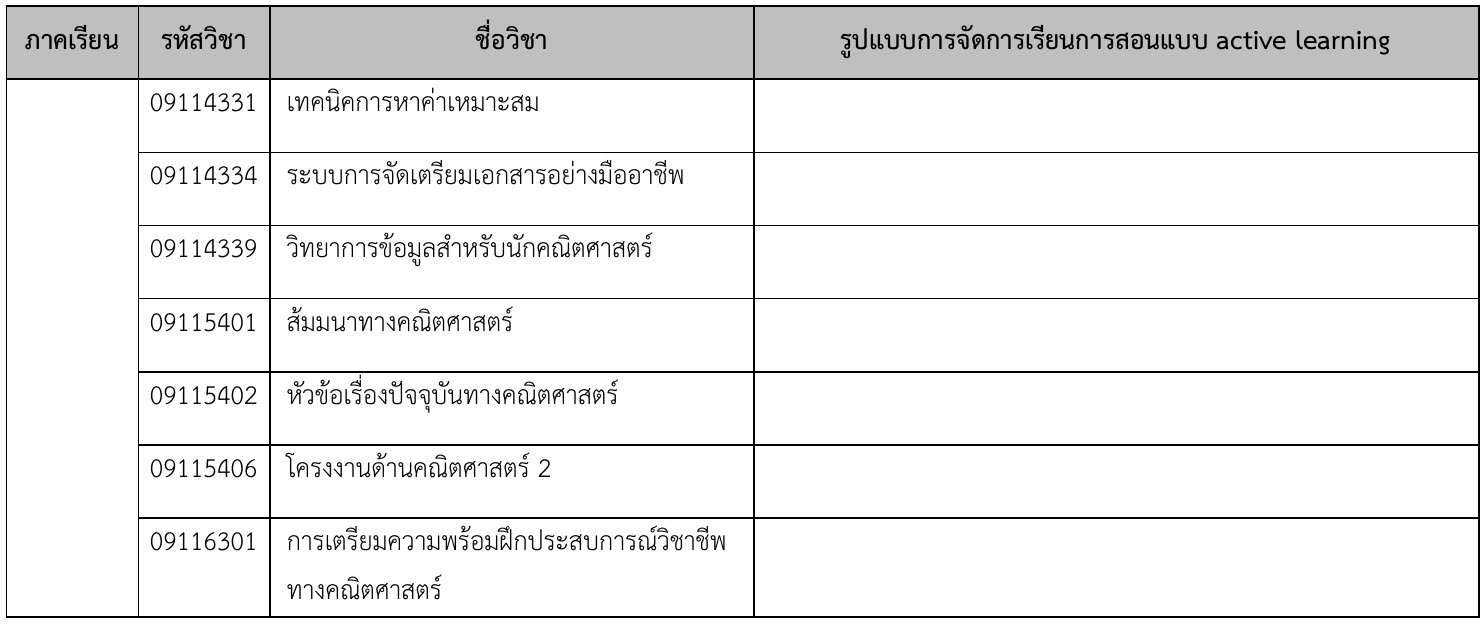
\includegraphics[width=1.05\textwidth]{Table3.3-2.jpg}
%\end{figure}
%\end{center}

\begin{doclist}
	\docitem{มคอ.3 }
	%\docitem{รูปแบบของการจัดการเรียนการสอนแบบ active learning ของแต่ละรายวิชาในหลักสูตร}
\end{doclist}


\subcriteria{The teaching and learning activities are shown to promote learning, learning how to learn, and instilling in students a commitment for life-long learning (e.g., commitment to critical inquiry, information-processing skills, and a willingness to experiment with new ideas and practices).}

เนื่องจากการสอนด้วยวิธีการ Active Learning จะทำ ให้ผู้เรียนเกิดแรงจูงใจในการเรียนรู้มากขึ้น  โดยผู้สอน
เป็นผู้อำนวยความสะดวก แนะนำ ช่วยเหลือสนับสนุนการเรียนรู้ ส่งผลทำให้เกิดบรรยกาศการเรียนการสอนที่ดีขึ้น ช่วยให้
ผู้เรียนเข้าใจบทเรียน สนใจ และเพิ่มแรงจูงใจให้กับผู้เรียนในการเรียนรู้ 
ดังนั้นหลักสูตรจึงส่งเสริมให้ทุกรายวิชามีการจัดการเรียนการสอนแบบ Active Learning เพื่อเป็นการสนับสนุนการเรียนรู้ให้กับนักศึกษา

หลักสูตรมีการส่งเสริมการเรียนรู้ตลอดชีวิต (life-long learning) ให้กับนักศึกษาในด้าน ทักษะการสืบค้นข้อมูล ความเป็นผู้นำ และการทำงานเป็นทีม โดยหลักสูตรฯ กำหนดให้ทุกรายวิชามีการส่งเสริมการเรียนรู้ตลอดชีวิตในด้านดังกล่าวให้กับนักศึกษา

%%%%%%%%%%%%%%




\begin{doclist}
	\docitem{มคอ.3 ของแต่ละรายแต่รายวิชา}
	\docitem{รายงานการประชุมอาจารย์ผู้รับผิดชอบหลักสูตร/อาจารย์ประจำสาขาวิชา การจัดการเรียนการสอนรายวิชาสัมมนา และการกำหนด Life-Long Learning ของหลักสูตร}
\end{doclist}


\subcriteria{The teaching and learning activities are shown to inculcate in students, new ideas, creative thought, innovation, and an entrepreneurial mindset.}

หลักสูตรมีการจัดกิจกรรมการเรียนการสอนเพื่อปลูกฝังให้ผู้เรียนมีความคิดใหม่ ๆ มีความคิดสร้างสรรค์ และมีแนวคิดการสร้างนวัตกรรม เช่น รายวิชาโครงงาน รายวิชาอัตลักษณ์แห่งราชมงคลธัญบุรี รายวิชา การคิดเชิงออกแบบ และรายวิชาสหกิจศึกษา เป็นต้น

หลักสูตรส่งเสริมแนวคิดการเป็นผู้ประกอบการ โดยจัดให้นักศึกษาเรียนรายวิชา 00-100-301 ความเป็นผู้ประกอบการ ซึ่งเป็นรายวิชาที่ศึกษาเกี่ยวกับแนวโน้มและแนวคิดในการทำธุรกิจ การเป็นผู้ประกอบการ การจัดการองค์กร การตลาด การจัดการด้านการเงิน การเป็นผู้ประกอบการที่ประสบความสำเร็จ การจัดทำแบบจำลองธุรกิจ
 
\begin{doclist}
	\docitem{ตัวอย่าง มคอ.3 รายวิชาที่ส่งเสริมแนวคิดการสร้างนวัตกรรมและแนวคิดความเป็นผู้ประกอบการ}
\end{doclist}

\subcriteria{The teaching and learning processes are shown to be continuously improved to ensure their relevance to the needs of industry and are aligned to the expected learning outcomes.}

หลักสูตรมีการปรับปรุงกระบวนการและกลยุทธ์การจัดการเรียนการสอนอย่างต่อเนื่องเพื่อให้แน่ใจว่ามีความสอดคล้องกับความต้องการของอุตสาหกรรมหรือสถานประกอบการและสอดคล้องกับผลการเรียนรู้ที่คาดหวัง โดยหลักสูตรได้ส่ง มคอ.3 รายวิชาระเบียบวิธีเชิงตัวเลขเบื้องต้นและรายวิชาระบบฐานข้อมูล ให้ผู้เชี่ยวชาญจากภาคอุตสาหกรรมให้ข้อเสนอแนะเกี่ยวกับกิจกรรมการเรียนการสอนในรายวิชาดังกล่าว โดยมีข้อเสนอแนะคือ หลักสูตรควรเพิ่มกิจกรรมการเรียนการสอนแบบเน้นปฏิบัติ ควรมีการนำกรณีศึกษาและปัญหาจากสถานประกอบ ให้นักศึกษาได้แก้ปัญหาจริง หรือควรเชิญผู้เชี่ยวชาญจากสถานประกอบการมาให้ความรู้ เพื่อให้เห็นความเชื่อมโยงระหว่างเนื้อหาที่เรียนในห้องเรียนกับการนำไปใช้จริงในสถานประกอบการ 

ผู้สอนในรายวิชาาระเบียบวิธีเชิงตัวเลขเบื้องต้นและรายวิชาระบบฐานข้อมูลได้นำข้อเสนอแนะมาปรับปรุงกิจกรรมการเรียนการสอนโดยมีการจัดกิจกรรมการเรียนการสอนแบบ Active Learning ในบางหัวข้อ และได้เชิญผู้เชี่ยวชาญจากสถานประกอบการคือ นายจิรพัฒน์ ลิ้มธนกุล ตำแหน่ง Senior Engineer Western Digital Storage Technology (Thailand) มาให้ความรู้ในหัวข้อ Python for industrial and application ในรายวิชาระเบียบวิธีเชิงตัวเลขเบื้องต้นและรายวิชาระบบฐานข้อมูล 




\begin{doclist}
	\docitem{มคอ.3 รายวิชาระเบียบวิธีเชิงตัวเลขเบื้องต้นและรายวิชาระบบฐานข้อมูล}
	\docitem{ภาพกิจกรรมการบรรยายหัวข้อ Python for industrial and application}
\end{doclist}

